%!TEX root=document.tex

\section{Introduction}
\label{sec:introduction}
\agp{We need to be careful about the use of: analyst vs. user, utility vs. scoring
function, ...}
Data visualization is often the first step in data analysis.
Given a new dataset or a new question about an existing dataset, an analyst builds
various visualizations to get a ``feel'' for the data, to find anomalies and outliers, 
and to identify trends and patterns that might merit further investigation. 
However, when working with high-dimensional datasets, identifying visualizations that
show interesting variations and trends in the data is non-trivial:
the analyst must manually specify a large number of visualizations, explore behavior of various
attributes (and combinations thereof), and examine different subsets of data before finally 
arriving at visualizations that depict something ``interesting'' or ``different''.
This need to manually specify and examine every visualization hampers rapid analysis 
and exploration of data.

In this paper, we tackle the problem of automatically identifying and recommending 
``useful'' or ``interesting'' visualizations to support fast visual analysis (we call these {\em high-utility visualizations}).
The goal of recommending high-utility visualizations brings up several challenges: first,
the curse of dimensionality makes the number of possible visualizations very large;
second, evaluating the utility of many visualizations by repeatedly re-running computations over the 
same underlying data is expensive; 
third, recommendations must be made to users in real-time, and at interactive speeds;
and fourth, identifying an {\em all-encompassing} scoring function for visualization utility is difficult. 
Our system, \SeeDB, is designed to address all of these challenges.

We begin with an illustrative example that explains the \SeeDB use case and motivates our
scoring function. 

% In this work, we combine an {\em incremental view pruning} framework with multi-
% query processing techniques to make recommendations in real time.
% As a first step towards crafting a sophisticated visualization scoring function, we adopt
% a deviation-based metric to quantify the utility of visualizations.

% Data visualization is one of the most common techniques for identifying 
% trends and finding anomalies in data.
% However, with high-dimensional datasets, identifying visualizations that 
% effectively present interesting variations or patterns in the data is a non-trivial task:  a
% user typically builds a large number of visualizations optimizing for a range of visualization 
% types, aesthetic features, and more
% before arriving at one that shows something valuable.

% In this paper, we tackle the problem of automatically recommending such valuable visualizations.
% The problem of recommending visualizations is complicated because a ``good'' visualization needs to take into account several different dimensions, including:
% \begin{inparaenum}
% \item types and properties of the different attributes in the dataset ({\it metadata}), 
% \item visual qualities of the visualization ({\it aesthetics}). 
% \item the particular subset of data the user is interested in ({\it query}), 
% \item variation in and distribution of the data itself ({\it data distribution}), 
% \item meaning and relative importance of attributes in the data ({\it semantics}),  and
% \item past history of interactions with this user and other users ({\it user preferences})
% \end{inparaenum}

% Current visualization systems like Spotfire and Tableau have limited capabilities to recommend visualizations --- they only focus on metadata and aesthetics dimensions, following standard visualization best-practices, e.g., choice of appropriate colors,
% rules defining when a bar chart is more appropriate than a trend line, etc.  
% No existing system that we are aware of 
% incorporates insights about the underlying data, or for that matter, any of the other dimensions into its recommendations.

%There is much room for research into leveraging information along the remaining dimensions to make more holistic
%recommendations.



%Data analysts must sift through very large volumes of data 
%to identify trends, insights, or anomalies.  This task often involves the visual inspection of data, 
%Given the scale of data, and the relative ease and intuitiveness of examining data visually,
%analysts often use visualizations as a tool to identify patterns of interest.
%Consequently, visualization software such as Tableau~\cite{}, Spotfire~\cite{} and Many Eyes~\cite{} 
%has seen unprecedented user adoption~\cite{kristi-tech-report}.
%In spite of user friendly software, however, selecting the ``right'' visualization still remains a laborious and 
%challenging task, particularly for novices unfamiliar with the data\mpv{citation?}. 
%As demonstrated by the paper on the Tableau use, majority of an analyst's time is spent in exploring
%different visualizations.
%To alleviate this problem, major visualization software vendors are attempting to incorporate automatic visualization
%recommendations into their software.
%For instance, Spotfire recently launched a ``Recommendations'' module that uses attribute metadata (e.g. type, number of distinct
%values) to suggest some ``best-practice'' visualizations~\footnote{http://spotfire.tibco.com/recommendations}.
%Similarly, Tableau's Show Me capability recommends a chart type (bar chart, map etc.) that is appropriate
%for the particular view of the data~\cite{DBLP:journals/tvcg/MackinlayHS07}.
%Both of these recommendations are straightforward applications of the best practices of visual design~\cite(); 
%neither incorporates insights about the underlying data or prior user history into its recommendations.
% These recommendations use basic metadata about attributes (categorical or numeric, number of distinct values etc)
% to produce simple visualizations that follow best practices of visual design.
%The ultimate vision for such a recommendation module is that given a dataset or a query, the visualization 
%software can study trends in data and previous interactions on that dataset to present to the user the 
%visualizations it deems most valuable.


% \mpv{Should we add a paragraph and schematic of an ideal system, that has an ensemble of models along one or 
% more of the above dimensions to produce a holistic list of recommendations?}

%In this paper, we develop a system that uses a combination of metadata, query, and statistics to 
%provide high quality, data-driven visualization recommendations.
%We envision our model to be used in conjunction with models currently used for recommendation and models that
%leverage context and user history to produce holisitc recommendations.

% \stitle{Data-driven Recommendations in \SeeDB.}
% To this end, in this work, we describe a new visualization recommendation engine we are building called {\it \SeeDB}.
% Eventually, we aim to address all six dimensions of the above list of dimensions by developing a suite of optimization techniques designed to explore
% the entire range of visualizations of a user-supplied data set or query result.  
% As a first step in this paper, we develop a general data-driven deviation-based metric that can capture all six dimensions to a limited extent (see Section~\ref{sec:problem_statement} and Section~\ref{sec:discussion}).  
% We focus on the query and data distribution aspects as a special case:
% these add significant utility, and at the same time significant complexity to 
% the visualization recommendation process,
% and are particularly relevant when an analyst is approaching a dataset 
% for the first time. 
% We leverage lessons from metadata and aesthetics-based recommendation
% generation from prior work.

% However, because metadata and aesthetics based recommendations have been addressed in prior work, in this paper we focus on {\it data-driven} recommendations that use information about data distribution, metadata and the user query to recommend visualizations.
% Such visualizations are particularly appropriate when
% approaching a dataset for the first time, with limited domain knowledge or historical context.

% that identify unusual variations in the result of the user-supplied query as compared to the underlying data.
% consider the inherent variations in the data from a user-supplied query. 
%   that focuses less on the aesthetics of good visualizations, and more
% on developing general techniques that explore the space
%of possible visualizations and recommend those that highlight data variability in the subset of data specified by a user's query.
%Metadata about a dataset, the user's query and information about data distributions can together provide powerful
%information to identify potentially interesting visualizations for the user.
%We call these recommendations {\it data-driven} since they do not draw upon any semantic information about the dataset;
%they are guided by statistics alone.
%We envision these techniques being incorporated into existing visualization systems that allow users to supply context (via, e.g.,
%interaction), and that focus more on the aesthetics of good visualization.
%As mentioned before, since we envision these recommendations to be augmented with context information (along with
%information about aesthetics), we can attack the problem piecemeal.

%Of course,  however, we note upfront
%that {\it there is a variety of ways to quantifying utility and these merit further exploration}.
%\mpv{In fact, we hope that the techniques and framework we describe in subsequent sections may be a general framework 
%into which we can plug in a variety of metrics.}

% deviation-based 

%%%%% VLDB original %%%%%%%

% \stitle{Illustrative Example.}
% Consider a smartphone app analytics team that is tasked with studying the metrics for BadApp, a smartphone app that has
% poor performance and has received a lot of consumer complaints. 
% Suppose that the team uses the AppMetrics database containing metrics such as network usage, 
% power consumption, load times etc.
% Given the large size of the database (millions of records), an analyst will 
% overwhelmingly use visualization software to glean insights into the behavior of BadApp.

% In a typical workflow, an analyst would begin by using the program's GUI or a custom query language to execute the equivalent
% of the following SQL query and pull all BadApp metrics from the database. 
% \noindent 
% \begin{align*}
% & \tt Q \ \ = \ \ SELECT \ * \ FROM \ \  AppMetrics \ \ WHERE  \ Name=``BadApp"
% \end{align*}
% Next, the analyst would use an interactive drag-and-drop GUI interface to visualize various metrics of BadApp.
% For instance, the analyst may visualize average network usage for BadApp, total crashes grouped by session time,
% average load times by carrier, distribution of mobile operating systems, and so on.
% Under the hood, these visualization operations are essentially queries to the underlying data store and subsequent graphing of 
% the results.
% For example, the visualization for average load times by carrier is generated by running an operation equivalent to the
% SQL query (Q') shown below.
% %The result of this query is a two-column table that is very likely going to be viewed as a bar-char~\cite{vql, kristi}.
% Table \ref{tab:staplerX} and Figure \ref{fig:staplerX} respectively show an example of the results of Q' and a potential
% visualization.

% \noindent
% \begin{align*}
% & \tt Q' = SELECT \ \ carrier,\ AVG(load\_time) \ \ FROM \ \  AppMetrics \\
% & \tt \hspace{20pt} WHERE\ Name=``BadApp" \ \ GROUP  \ \ BY \ \ carrier
% \end{align*}

% \begin{figure}[h]
% \vspace{-10pt}
% 	\centering
% 	\begin{subfigure}{0.49\linewidth}
% 	   \begin{tabular}{cc} \hline
% 		  Carrier & Load Times (ms) \\ \hline
% 		  AT\&T & 180.55 \\ \hline
% 		  Sprint & 90.13 \\ \hline
% 		  T-Mobile & 122.00 \\ \hline
% 		  Verizon &  145.50\\ \hline
% 		  \end{tabular}
% 		  \caption{Data: Average Load Times by Carrier for BadApp} \label{tab:staplerX}
% 	\end{subfigure}
% 	\begin{subfigure}{0.49\linewidth}
% 		\centering
% 		{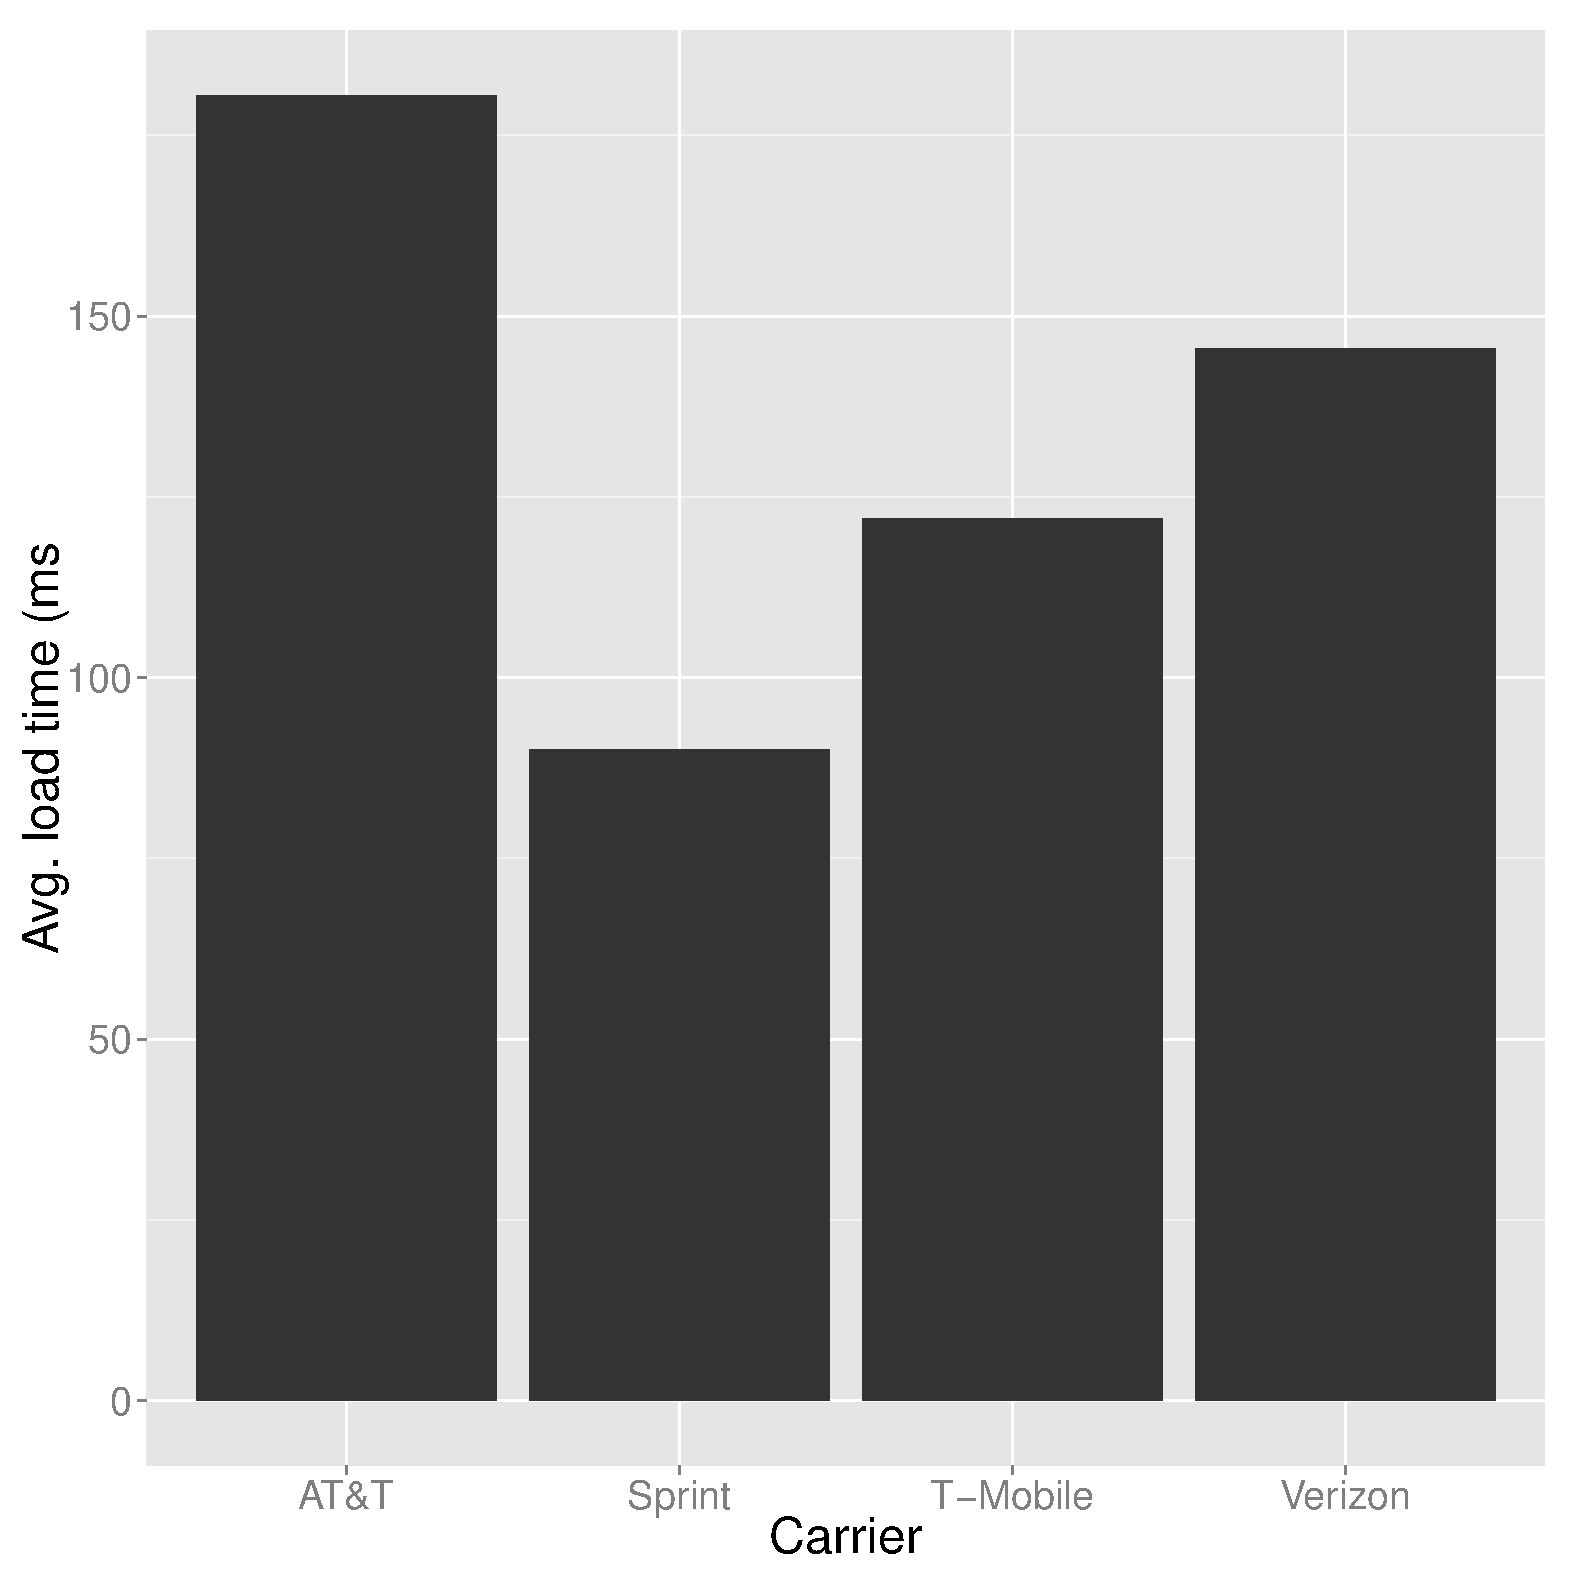
\includegraphics[width=4cm] {Images/dist1.pdf}}
% 		\caption{Visualization: Average \\ Load Times by Carrier
% 		 for BadApp}
% 		\label{fig:staplerX}
% 	\end{subfigure}
	
% 	\centering
% 	\begin{subfigure}{0.49\linewidth}
% 		{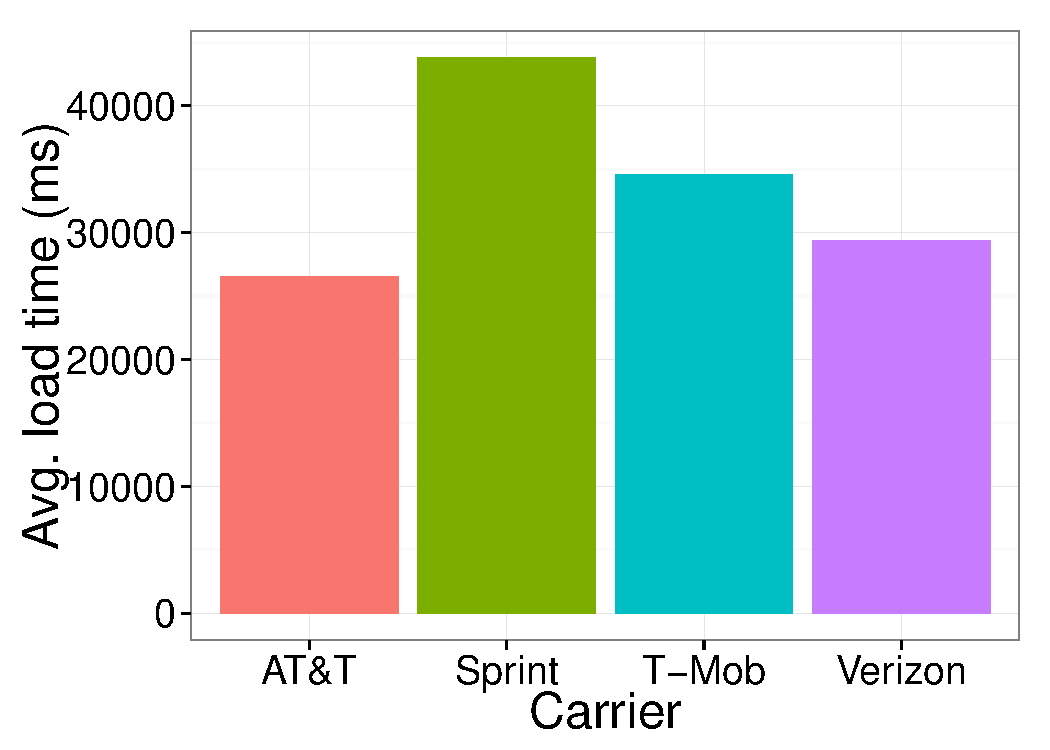
\includegraphics[width=4cm] {Images/dist2.pdf}}
% 		\caption{Scenario A: Average Load Times by Carrier}
% 		\label{fig:staplerX-a}
% 	\end{subfigure}
% 	\begin{subfigure}{0.49\linewidth}
% 		\centering
% 		{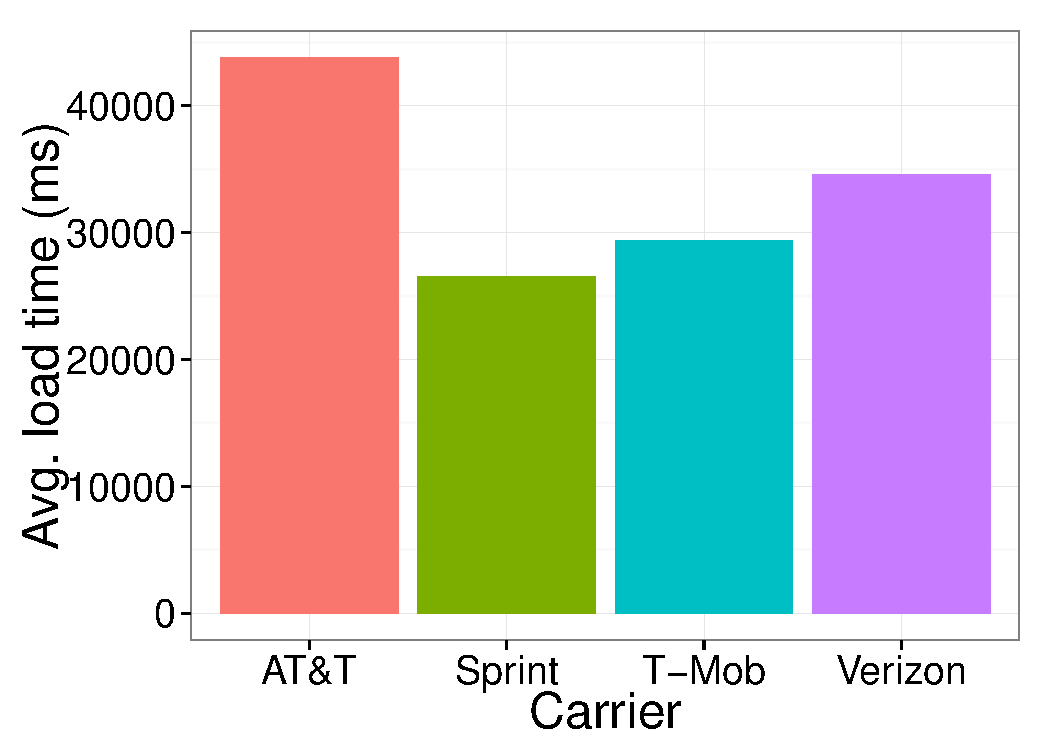
\includegraphics[width=4cm] {Images/dist3.pdf}}
% 		\caption{Scenario B: Average Load Times by Carrier}
% 		\label{fig:staplerX-b}
% 	\end{subfigure}
% 	\vspace{-10pt}
% 	\caption{Motivating Example}
% 	\label{fig:intro}
% 	\vspace{-15pt}
% \end{figure}

%%%%%% VLDB original end %%%%%%%

\reviewer {
	W2: Using the illustrative example is helpful, but would have been even more
helpful if it would be based on a real dataset actually used in the evaluations. 
Using the illustrative example was helpful and quite motivating.
However, this introduced another dataset not used in the evaluations
afterwards. To use a dataset, which was actually used in the evaluation would
make the presentation more coherent. Figure 1 uses the BadApp dataset,
Figure 3 a donation dataset, then other datasets are introduced for the
evaluation, and the diabetes dataset for the user studies. Focusing on the
diabetes dataset in Figure 1 and Figure 3 would leave more room to reuse
them to discuss some findings for example using Figure 3.
}
\mpv{sure, if we have time} \agp{I think this is worth investing 
the time in--shouldn't take more than half an hour to dig up, right? We can
also point at these visualizations and say that these were actually
returned by \SeeDB.}
\srm{I agree!}


\begin{example}
Consider a smartphone app analytics team that is tasked with answering why a certain app, 
BadApp, is showing poor performance and receiving consumer complaints. 
Suppose that the team uses the AppMetrics database containing metrics such as network usage, 
power consumption, and load times to perform the analysis.
The analyst begins by querying the AppMetrics database for BadApp-specific data and uses her 
favorite visualization software to graph various metrics for BadApp.

For instance, she may visualize average network usage for BadApp, 
correlation between session times and number of crashes, average load times by carrier, 
comparison of mobile operating systems running BadApp vs.~other apps, and so on,
in order to identify what metrics BadApp may be misbehaving on.
Depending on the types of visualizations created, the number of possible 
visualizations grows exponentially with the number of metrics in the database.
\agp{What do you mean by this?}
Clearly, beyond a small number of metrics, creating and examining all possible visualizations
becomes untenable.
% For example, the visualization for average load times by carrier is generated by running an operation equivalent to the
% SQL query (Q') shown below.
% %The result of this query is a two-column table that is very likely going to be viewed as a bar-char~\cite{vql, kristi}.
% Table \ref{tab:staplerX} and Figure \ref{fig:staplerX} respectively show an example of the results of Q' and a potential
% visualization.

% \noindent
% \begin{align*}
% & \tt Q' = SELECT \ \ carrier,\ AVG(load\_time) \ \ FROM \ \  AppMetrics \\
% & \tt \hspace{20pt} WHERE\ Name=``BadApp" \ \ GROUP  \ \ BY \ \ carrier
% \end{align*}



\begin{figure}[h]
\vspace{-10pt}
	\centering
	\begin{subfigure}{0.49\linewidth}
	   \begin{tabular}{cc} \hline
		  Carrier & Load Times (ms) \\ \hline
		  AT\&T & 180.55 \\ \hline
		  Sprint & 90.13 \\ \hline
		  T-Mobile & 122.00 \\ \hline
		  Verizon &  145.50\\ \hline
		  \end{tabular}
		  \caption{Data: Average Load Times by Carrier for BadApp} \label{tab:staplerX}
	\end{subfigure}
	\begin{subfigure}{0.49\linewidth}
		\centering
		{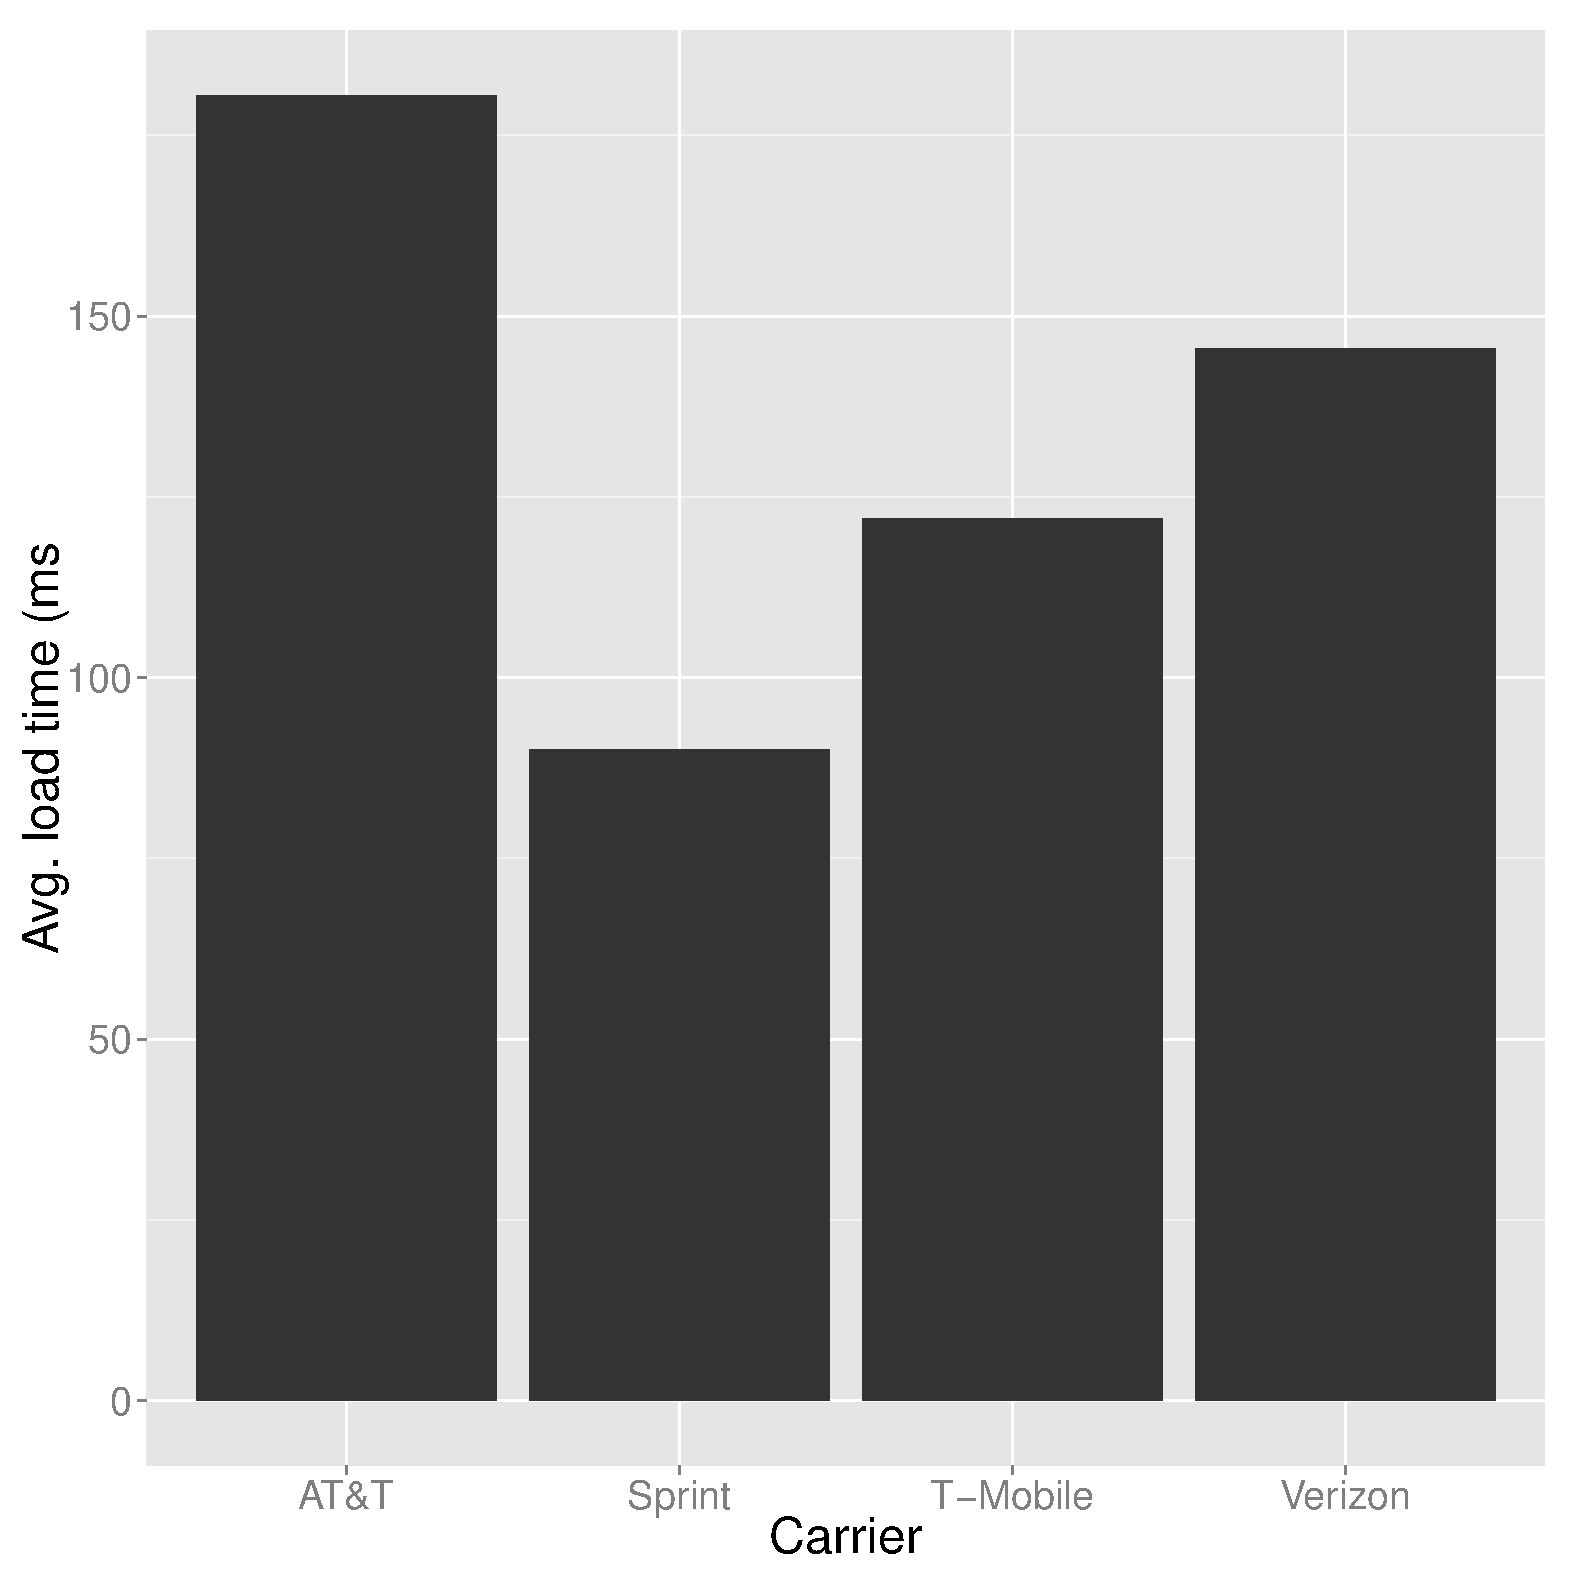
\includegraphics[width=4cm] {Images/dist1.pdf}}
		\caption{Visualization: Average \\ Load Times by Carrier
		 for BadApp}
		\label{fig:staplerX}
	\end{subfigure}
	
	\centering
	\begin{subfigure}{0.49\linewidth}
		{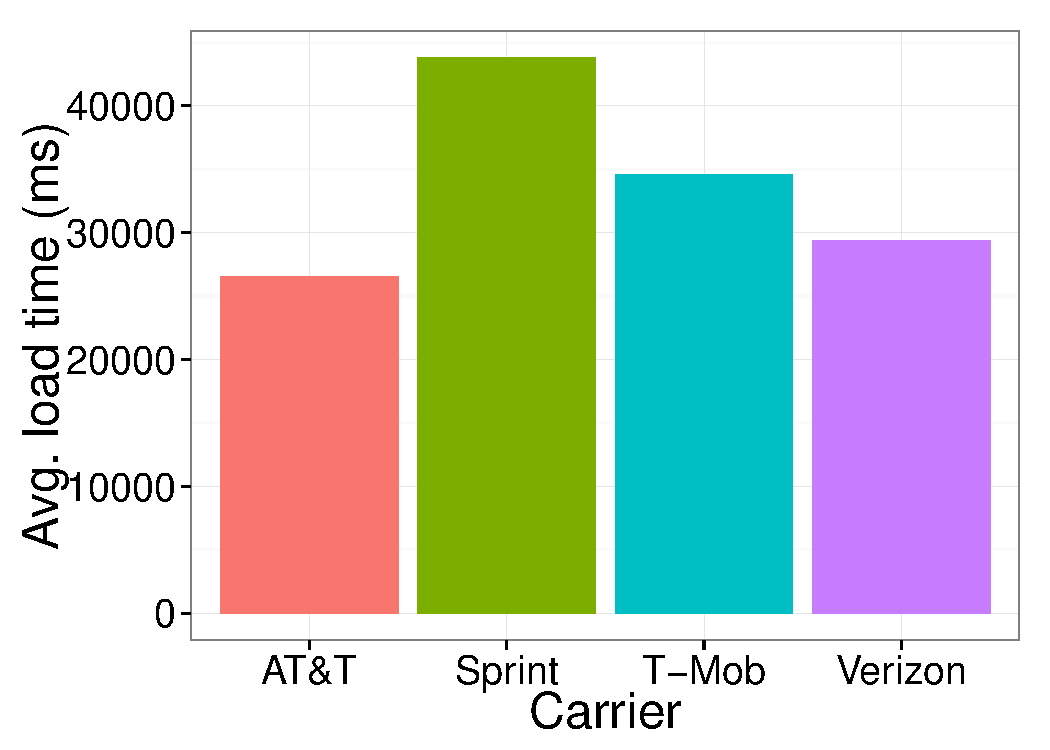
\includegraphics[width=4cm] {Images/dist2.pdf}}
		\caption{Scenario A: Average Load Times by Carrier}
		\label{fig:staplerX-a}
	\end{subfigure}
	\begin{subfigure}{0.49\linewidth}
		\centering
		{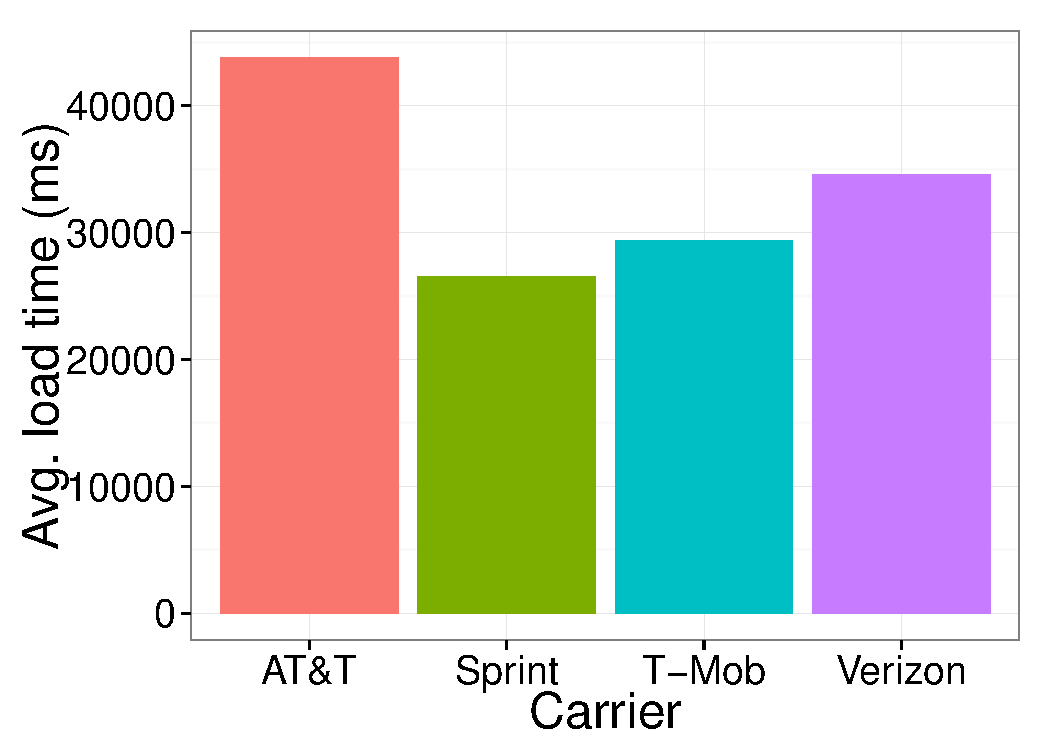
\includegraphics[width=4cm] {Images/dist3.pdf}}
		\caption{Scenario B: Average Load Times by Carrier}
		\label{fig:staplerX-b}
	\end{subfigure}
	\vspace{-10pt}
	\caption{Motivating Example}
	\label{fig:intro}
	\vspace{-15pt}
\end{figure}

What might make one of these visualizations ``interesting'' or valuable for the 
task at hand depends on a number of factors.
For a task like the one described above, we posit that 
{\em a visualization is 
potentially ``interesting'' if it shows
a trend that deviates from the expected trend}.
In our metric, the expected trend is the trend we observe on the entire data (i.e. metrics for
all apps), while the real trend is the trend we observe in the data being analyzed (i.e. 
metrics for BadApp).
Deviations of the real trend from the expected trend make a visualization interesting.
\srm{ I don't like the words ``trends'' or ``expected'' here.  Trend suggests some kind of time series.  And how do
we know what the user expects??? }
Therefore, the visualization of load times by carrier, as shown in Figure
\ref{fig:staplerX}, would be interesting if the trend for load times across all
apps showed the {\it opposite} trend (e.g. Figure \ref{fig:staplerX-a}), and would
be uninteresting if the overall trend for all apps followed a similar trend 
(Figure \ref{fig:staplerX-b}).
\end{example}



\mpv{acknowledge that this is from the vision paper?}
\mpv{Say that metric is suited to when there user is unfamiliar with the data, cold
starts?}

\agp{We need to articulate that our goal is to build \SeeDB that actually makes
these recommendations.}
Since our goal with \SeeDB is to make visual analytics faster, we adopt a metric
that prefers visualizations that show interesting or surprising trends in data.
Specifically, we are motivated by the following observation:
\begin{quotation}
The greatest value of a picture is when it forces us to notice what we never expected to see.
\end{quotation} 
\begin{flushright} 
- John Tukey, Exploratory Data Analysis 1977
\end{flushright}
We formally define the deviation-based scoring function in the next section. 

% While this utility metric is an example of a simple recommendation metric,
% it plays an important role in recommendations when 
% there is no prior history --- and therefore no user preferences
% or understanding of context.
% This special case is especially appropriate when the analyst
% is not very familiar with a dataset and is analyzing it for the first time.
% That said, in Section~\ref{sec:discussion}, we describe how our deviation-based
% metric can, in fact, encompass a large number of data-driven utility metrics and
% can be seamlessly extended to support other dimensions such as user preferences.

In addition to our deviation-based metric, there are other dimensions and
functions that can be used to score visualization utility.
These include other functions based on data distribution (e.g. scoring based on 
statistical summaries) and functions that measure utility along {\em 
dimensions} other than data distribution. 
These utility dimensions 
include aesthetics (e.g. is a bar plot more appropriate than a 
scatter plot), context (e.g. prior knowledge that only female patients visit the
obstetrics department), and user preference (e.g. in the sales dataset, profit is
the most relevant attribute).
Exploration of each of these dimensions forms a distinct body of work.
We leave a detailed investigation of these dimensions for future work, but 
outline in Section \ref{sec:discussion} 
our initial attempts at extending \SeeDB to support them.

% functions 
% that can be used to score the utility of a 
% visualization; these can be different functions based on data distribution (e.g. scoring
% based on statistical summaries of data or outlier detection) or functions that take
% orthogonal {\em dimensions} of utility into account, e.g., user preferences, aesthetics, and context.
% The pruning framework we propose in Section \ref{sec:in_memory_execution_engine} can be applied to a large set of 
% functions derived from data distribution, and \SeeDB
% can support these metrics without any changes. \mpv{Verify true? Add characterization
% of metrics}
% Investigations of the other dimensions of utility form a distinct body of work, and
% we leave these explorations for future work.
% \mpv{keep? In section \ref{sec:discission}, we outline some means by which \SeeDB may be 
% extended to support these metrics.}
% We leave the investigation of other dimensions of utility to future work, but outline
% in Section \ref{sec:discussion} some means by which \SeeDB may be extended to support them.

% Due to the scale of data, most common visualizations show aggregate summaries of data
% as opposed to individual records (e.g. average sales by state vs. sales of each store 
% in every state).
% Consequently, our current implementation of \SeeDB\ recommends visualizations that show aggregate 
% summaries of data.

% Of course, there are a variety of other possible data-driven metrics for quality or utility
% of a visualization.
% For instance, one might focus on visualizations that show order statistics or anomalies~\cite{DBLP:conf/avi/KandelPPHH12}. 
% These would be important for spotting, for example, unusual spikes in machine load.
% Similarly, drawing upon the literature on data cubes, one might choose visualizations that highlight aggregates that
% are unusual given the remaining values in the cube~\cite{DBLP:conf/vldb/Sarawagi00}.
% Finally, one might choose to not aggregate any values but show correlations between attributes by plotting a random
% sampling of data-points.  Incorporating these other types of visualizations into our framework is an interesting
% direction for future work.

\reviewer{
	The method does not consider the context, semantics, and any user
preferences all important components of viz	
}
\mpv{Yeah I say that above. Any additions?}



% The majority of visualizations that are generated in visualization systems are based on aggregate summaries of the
% underlying data.
% As a result, the {\it trends} we study are the results of grouping and aggregation applied to a given dataset.


% Thus, the recommendation algorithm used by \SeeDB\ works as follows: given a dataset $D$ and a query $Q$
% indicating the subset of data of interest to the analyst, \SeeDB finds the visualizations of $Q$ that 
% show the highest deviation between trends in $Q$ and trends in $D$. 
% Specifically, \SeeDB considers visualizations that can be constructed via a combinations of grouping and 
% aggregation applied to $Q$.

No current system is that we are aware of makes use of variation in the underlying
data to recommend visualizations. \srm{Cite heer's recent work?}
 Current visualization packages like Spotfire and Tableau have limited capabilities for 
recommending visualizations.
Their recommendations only implement rules-of-thumb regarding chart aesthetics such as choice of
chart type, colors and marks.
%No existing system that we are aware of leverages insights about the underlying data
%into make visualization recommendations. \mpv{does this sound ok?} \agp{I would start with
%the statement that no current system supports the recommending of interesting visualizations
%where the target dataset shows some discrepancies not found in the underlying data.
%Then say the first two lines.}

In the following sections, we propose a general-purpose view pruning framework and a set
of multi-query optimization techniques that make responses possible in real time.
We then present exerimental evaluation of \SeeDB via both a performance study and a user study.
In summary, the contributions of this paper are:

% efficiently manages the search
% for data-driven visualization recommendations at interactive time scales.
% We show that \SeeDB can be implemented on top of a traditional relational database,
% allowing it to take advantage of the benefits of the interfaces and features
% relation engines expose.
% Doing this, however,
% also leads to inefficiencies that arise due to the requirement that data be
% accessed via SQL.   
% We manage these inefficiencies by introducing two classes of optimizations:
% {\em sharing-based} optimizations, that try to batch
% and share as much computation as possible to minimize the number of SQL queries,
% and {\em pruning-based optimizations}, that try to avoid
% as much unnecessary work as possible, and discarding candidate aggregate views
% that are of low utility.

\mpv{revisit contributions} \agp{The order of this is off.}
\begin{denselist}
%  \item We design \SeeDB as a system for data-driven visualization recommendations.
%  We explore and evaluate two distinct implementations of the system, one as a
%  wrapper around a database and another a custom solution (Section~\ref{sec:system_architecture}).
  \item We present \SeeDB, a visualization recommendation system that can run
  as a middleware layer on any SQL-compliant DBMS (Section~\ref{sec:system_architecture}).
  \item We adopt and evaluate a deviation-based scoring function for measuring utility
  of a visualization (Section~\ref{sec:problem_statement}).
  \item We propose a set of multi-query optimization techniques which in combination
  with the pruning framework maximize the sharing of computation between visualization
  computations (Section~\ref{sec:sharing_opt}).
  \item We propose a general-purpose view pruning framework to quickly identify
  high-utility visualizations by adapting techniques from traditional 
  confidence-interval-based~\cite{hoeffding1963probability} top-$k$ ranking and the
   multi-armed bandit problem~\cite{bandits} (Section~\ref{sec:in_memory_execution_engine}).
  % \item We describe a general deviation-based framework 
  % for evaluating the utility  of a visualization,
  % and present and evaluate a specific metric that identifies 
  % aggregate dimensions in a dataset that
  % show maximal variation (Section~\ref{sec:problem_statement}).
  % We develop two classes of optimizations to make such aggregates run fast 
  % in a conventional DBMS.
  % \item The first set of techniques
  % combine queries and aggregates to minimize the number of queries executed and 
  % maximize the sharing of scans between queries, 
  % including bin-packing~\cite{garey} algorithms and parallelization
  % (Section~\ref{sec:sharing_opt}).
  % \item The second set of techniques further optimize the process by adapting techniques 
  % from both traditional confidence-interval-based~\cite{hoeffding1963probability} top-$k$ ranking and the
  %  multi-armed bandit problem~\cite{bandits} 
  %  to the problem finding the top-$k$ visualizations (Section~\ref{sec:in_memory_execution_engine}).
  % \item We explore visualization pruning techniques based on data distribution
  % to prune visualizations even before they are evaluated by the \SeeDB\ system 
  % (Section~\ref{sec:pruning}).
  \item We evaluate the performance of our pruning framework and demonstrate that \SeeDB
  can identify high-utility visualizations with high accuracy. We also demonstrate that 
  our optimizations provide a 40-100X speedup on both relational row and column stores
  (Section~\ref{sec:experiments}). 
  \item We present the results of a user study evaluating the role of visualization 
  recommendations in visual analysis and the quality of \SeeDB recommendations in particular
  (Section \ref{sec:user_study}).
\end{denselist}

The vision for \SeeDB\ has been described in a vision paper~\cite{DBLP:conf/vldb/Parameswaran2013} and presented as demonstration~\cite{DBLP:journals/pvldb/VartakMPP14}, but neither of these short papers described detailed algorithms or
presented any form of evaluation.
Specifically, this work builds upon the \SeeDB vision by proposing a novel, general-purpose view 
pruning framework, a combination of multi-query optimization techniques, and presenting 
both a performance study of the system as well as a user study demonstrating the efficacy of our system in aiding analysis.
\reviewer{
	I like the ideas in this paper, but they have been presented in a vision paper
and demo paper. So to warrant a new publication the execution of these
ideas (the specific search techniques) and their evaluation need to be novel,
interesting, and well executed. I found the evaluation in particular to be
lacking.
}

\reviewer{
	This paper’s contribution seems to be mostly section 4.3 (pruning
optimizations) and the tests (Sections 5 and 6). The differences with
references [27] and [37] should be made more clear.
}


